\chapter{Durability Theory} \label{chap:kdur-theory}

In this chapter we use the results from Part 2 and background information of how MongoDB persists write operations to equip the reader with the tools to reason about varying levels of durability in a flexible manner by developing a novel theoretical model of when write durability occurs. This model will then allow the reader to understand the theoretical foundation on estimating when a write becomes durable using simple measurements present with each individual write operation.

We will begin with a discussion of the circumstances required to make a write durable and proceed to loosen those restrictions to introduce a more flexible form of write durability. We then compare this model to MongoDB's write concern and show that MongoDB's journaled write concern provides weaker guarantees compared to this model, concluding by showing how this model can be used to estimate when writes become durable.

\section{Introduction}
Upon closer inspection of the execution histories which contained lost writes, we notice that the writes that tended to be confirmed \textit{closer} to the time of failure were more likely to be lost. This leads us to believe that these writes were lost because no secondaries were informed of the operation prior to the failure.

\section{Total Durability}
In order to be absolutely certain that a write will not be lost even if \textit{all} nodes crash, we must allow the write to be propagated to and persisted by every node in a replica set $R$. 

Let us define $t$ as the time a write operation was submitted and $t_a$ as the time at which it has been persisted to all nodes. The time it takes for a write to be persisted is comprised of the time it takes for the node to receive the write and the time it takes for the write to be written into memory and flushed to disk. We will define these as $l$ and $d$ respectively. As such, for an individual node $r$, the time at which it persists the write to disk is $l_r + d_r$. An illustration of this process is seen in \prettyref{fig:write}. Assuming that all replicas will retrieve the write in parallel, we can say:
\begin{equation} \label{eq:ta}
    t_a = \max_{r \in R}(l_r + d_r) + t
\end{equation}

\begin{figure}
    \centering
    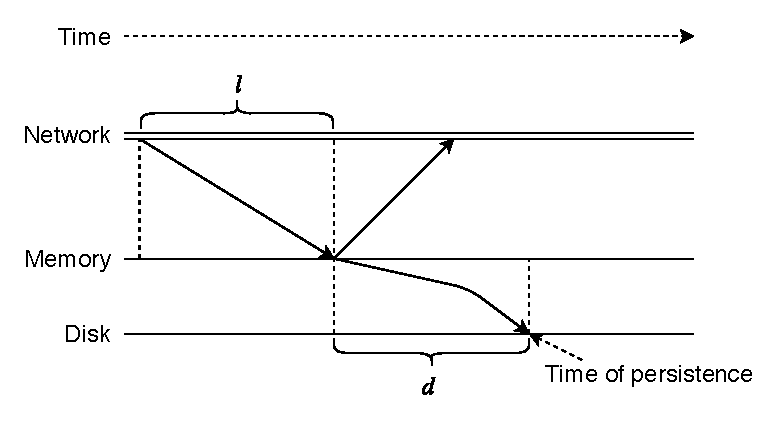
\includegraphics[width=\textwidth]{images/write.pdf}
    \label{fig:write}
    \caption{A time-space diagram of a write being persisted onto a single node}
\end{figure}

\section{K-Durability}

We now make a vital observation - if total durability is defined when \textit{all} replicas persist a write, we can define a measure for when $k$ replicas persist a write. 

We define a write as \textit{k-durable} if it has been persisted onto $k$ replicas. A k-durable write can sustain $k-1$ crashes and still be visible to the replica set after an election. Using this definition, and equation \prettyref{eq:ta} we derive the time at which a write becomes k-durable as: 
\begin{center}
\begin{equation} \label{eq:tk}
t_k = \max_{r \in R_k}(l_r + d_r) + t
\end{equation}
Where $R_k$ is the set comprised of the first $k$ nodes that have persisted the write.
\end{center}

We can now see that a totally durable write is $t_a = t_k$ where $k = |R|$. Intuitively, $t_k \leq t_a \ \forall k$ as we simply ignore the $|R| - k$ worst durations. This means that it is quicker for a write to become k-durable than totally durable.

This model can be used to predict the durability of any write as a function of the duration since the write was acknowledged. Specifically, if we can measure the probability distributions of $l$ and $d$, we estimate how many nodes have persisted the write at a given point in time, hence estimating the write's durability level.

\section{K-Durability \& Write Concern}
Recall from \prettyref{sec:writeconcern} that MongoDB's write concern configuration can specify how many replicas must acknowledge the write before the primary acknowledges it to the client. The write concern configuration can also specify whether a write is to be journaled, which should ensure that the operation is persisted before being acknowledged. Journaled write concern $k$ should then be a good approximation of $k$-durability - the operation is expected to have reached $k$ nodes and been persisted to the journal on all $k$ nodes prior to acknowledgement. 

However MongoDB buffers write operations before persisting them as a batch. The buffering behaviour compromises all durability assumptions as we \textit{cannot} guarantee that a write operation has been persisted when we receive an acknowledgement. 

\section{Estimating 1-durability}
Recall the definition of $k$-durability from equation \ref{eq:tk}. Substituting $k = 1$, we get the following:
\[
    t_1 = \max_{r \in R_1}(l_r + d_r) + t
\]
Now we observe that $R_1$ is a set consisting only of the first node that persists the operation. Recall that the primary replica will add the operation to its Oplog only \textit{after} persisting it. This means the secondary nodes will not even be aware of an operation until after the primary persists it. As such, the primary \textit{must} be the first node to persist the operation. Hence $R_1 = $ \{\textit{primary}\} and our equation for $t_1$ can be simplified as follows:
\begin{center}
\begin{equation} \label{eq:t1}
    t_1 = l_{\text{\textit{primary}}}+ d_{\text{\textit{primary}}} + t
\end{equation}
From here onwards, the \textit{primary} subscript will be left out for brevity.
\end{center}

As a result, to estimate 1-durability of an operation, it is sufficient to estimate when the primary persists the operation.

Recall that journaled write concern is supposed to act as a method for ensuring a write is persisted before acknowledgement. While this is not MongoDB's exact behaviour, as MongoDB buffers journaled operations before flushing them to disk, it is a good approximation. We define the time a journaled write gets acknowledged as:
\[
    j = 2l + d_{\text{\textit{est}}} + t
\]

We notice this is very similar to our definition of $t_1$ in equation \ref{eq:t1}. Therefore we define an estimate of 1-durability as:

\begin{equation} \label{eq:persist}
    t_{1\_est} = j - l
\end{equation}
We will now show that $t_{1\_est}$ is a valid approximation of $t_1$ using the measurements of ping latency $l$ and latency $j$ of a journaled write:
\begin{align*} 
    t_{1\_est} &= j - l \\
    &= l + d_{\text{\textit{est}}} + t \\
    &\approx l + d + t\\
    &\approx t_1
\end{align*}

As such we prove that we can use equation \ref{eq:persist} to estimate 1-durability of an operation.